\documentclass[ucs,10pt]{beamer}
\mode<presentation>
%\hypersetup{pdfpagemode=FullScreen}

\usepackage{beamerthemesplit}
\usepackage{beamer_visser_um}


\usepackage{tikz}   
\usepackage{subfigure}
\usepackage{multimedia}
\usepackage{tcolorbox}
\usepackage{array,tabularx}
\usepackage{colortbl}

\setlength{\unitlength}{\textwidth}  % measure in textwidths 

\setbeamertemplate{sidebar right}{}
\setbeamertemplate{footline}{%
\hfill\usebeamertemplate***{navigation symbols}
\hspace{1cm}\insertframenumber{}/\inserttotalframenumber}


\title{Activity Monitoring and Prediction for Humans and NAO Humanoid Robots using 
	Wearable Sensors}
\author{Saminda Abeyruwan, \underline{Faisal Sikder}, Ubbo Visser, and Dilip Sarkar}
\institute{Department of Computer Science\\ University of Miami \\ \vspace{.25cm}}
\date{May 19, 2015}
\titlegraphic{\putat{-0.52}{-0.15}{
\includegraphics[height=1.5cm]{logos/theUlogo}}}


\begin{document}

%%%%%%%%%%%%%%%%%%%%%%%%%%%%%%%%%%%%%%%%%%%%%%%%%%%%%%%%%%%%%


\frame{\titlepage}

%\section*{Outline}
%\frame{
%  \frametitle{Outline}    
%  \tableofcontents
%}


%%%%%%%%%%%%%%%%%%%%%%%%%%%%%%%%%%%%%%%%%%%%%%%%%%%%%%%%%%%%%

\section{Introduction}
\subsection{Introduction}

\frame{
  \frametitle{Introduction}
  \setbeamercovered{transparent} 
  
  \begin{tcolorbox}[colback=green!5,colframe=darkgreen!90!black,title=Challenges]
  \begin{itemize}
  	\item To distinguish between: 
	  	\begin{itemize}
	  		\item \textbf{Human}: daily activities and falls.
	  		\item \textbf{Humanoid robots}: normal motions and falls.
	  	\end{itemize}
	
	\item  To design and develop a unified platform for both. 
	    		
	\end{itemize}
  \end{tcolorbox}  
  
}

%%%%%%%%%%%%%%%%%%%%%%%%%%%%%%%%%%%%%%%%%%%%%%%%%%%%%%%%%%%%%
%\subsection{Motivation}
%\subsubsection*{Motivation}
%\frame{
%	\frametitle{Motivation}
%	\setbeamercovered{transparent}
%	\begin{tcolorbox}[colback=green!5,colframe=darkgreen!90!black,title=Motivation]
%	\begin{itemize}
%	\item Humans and biped humanoid robots have almost identical motions.
%	\item  Susceptible to 
%	similar accidents.
%	\item Same set of learning algorithms
%			 	are suitable for both groups.
% 	\item Off-the-shelf hardware components to develop our sensing tools.
% 	\item Generalized approach for learning and predicting
% 	activities of both groups.
% 	
% 	\item  Detection of falls for both humans and robots within a unified framework;
% 	
%	\end{itemize}
%	\end{tcolorbox}
%	
%}

%%%%%%%%%%%%%%%%%%%%%%%%%%%%%%%%%%%%%%%%%%%%%%%%%%%%%%%%%%%%%

\section{Our Approach and Contributions}
\subsection{Devices}
\subsection{Framework}
\subsection{Activity Annotation}

\frame{
	\frametitle{Our Approach and Contributions}
	\setbeamercovered{transparent}
	
	\begin{tcolorbox}[colback=green!5,colframe=darkgreen!90!black,title=Devices and Software Tools]
	\begin{itemize}
				\item Off the shelf hardware: 
				% one of the best availale with affordable price, with lot of features in it
				\begin{enumerate}
				\item Tiva C Series TM4C123G microcontroller board.
				\item Sensor Hub BoosterPack for sensing 9-axis motion.
				\item CC2533 BoosterPack for wireless networking.\\[2ex]
				\end{enumerate}
				\item Software tools developed:				
				\begin{enumerate}
					 \item Setup the wireless sensor network (WSN). 
					 \item Collect data using WSN. 
					 \item Learn to distinguish among events (such as walking forward, turn clockwise etc.).
					 \item Monitor and predict events. 
				\end{enumerate} 
			\end{itemize}
	\end{tcolorbox}
	 
	
}

\frame{
	\frametitle{Device Placement}
	\setbeamercovered{transparent} 
	\begin{figure}[!ht]
		\centering
		\minipage{0.48\textwidth}
		%\begin{tcolorbox}[colback=white!5,colframe=darkgreen!90!black]
			\centering \includegraphics[width=0.7\linewidth]{figures/human_figure}
			%\caption{5 Vs 5}\label{fig:timePlot}
		%\end{tcolorbox}
		\endminipage \hspace{2mm}
		\minipage{0.48\textwidth}
		%\begin{tcolorbox}[colback=white!5,colframe=darkgreen!90!black]
			\centering 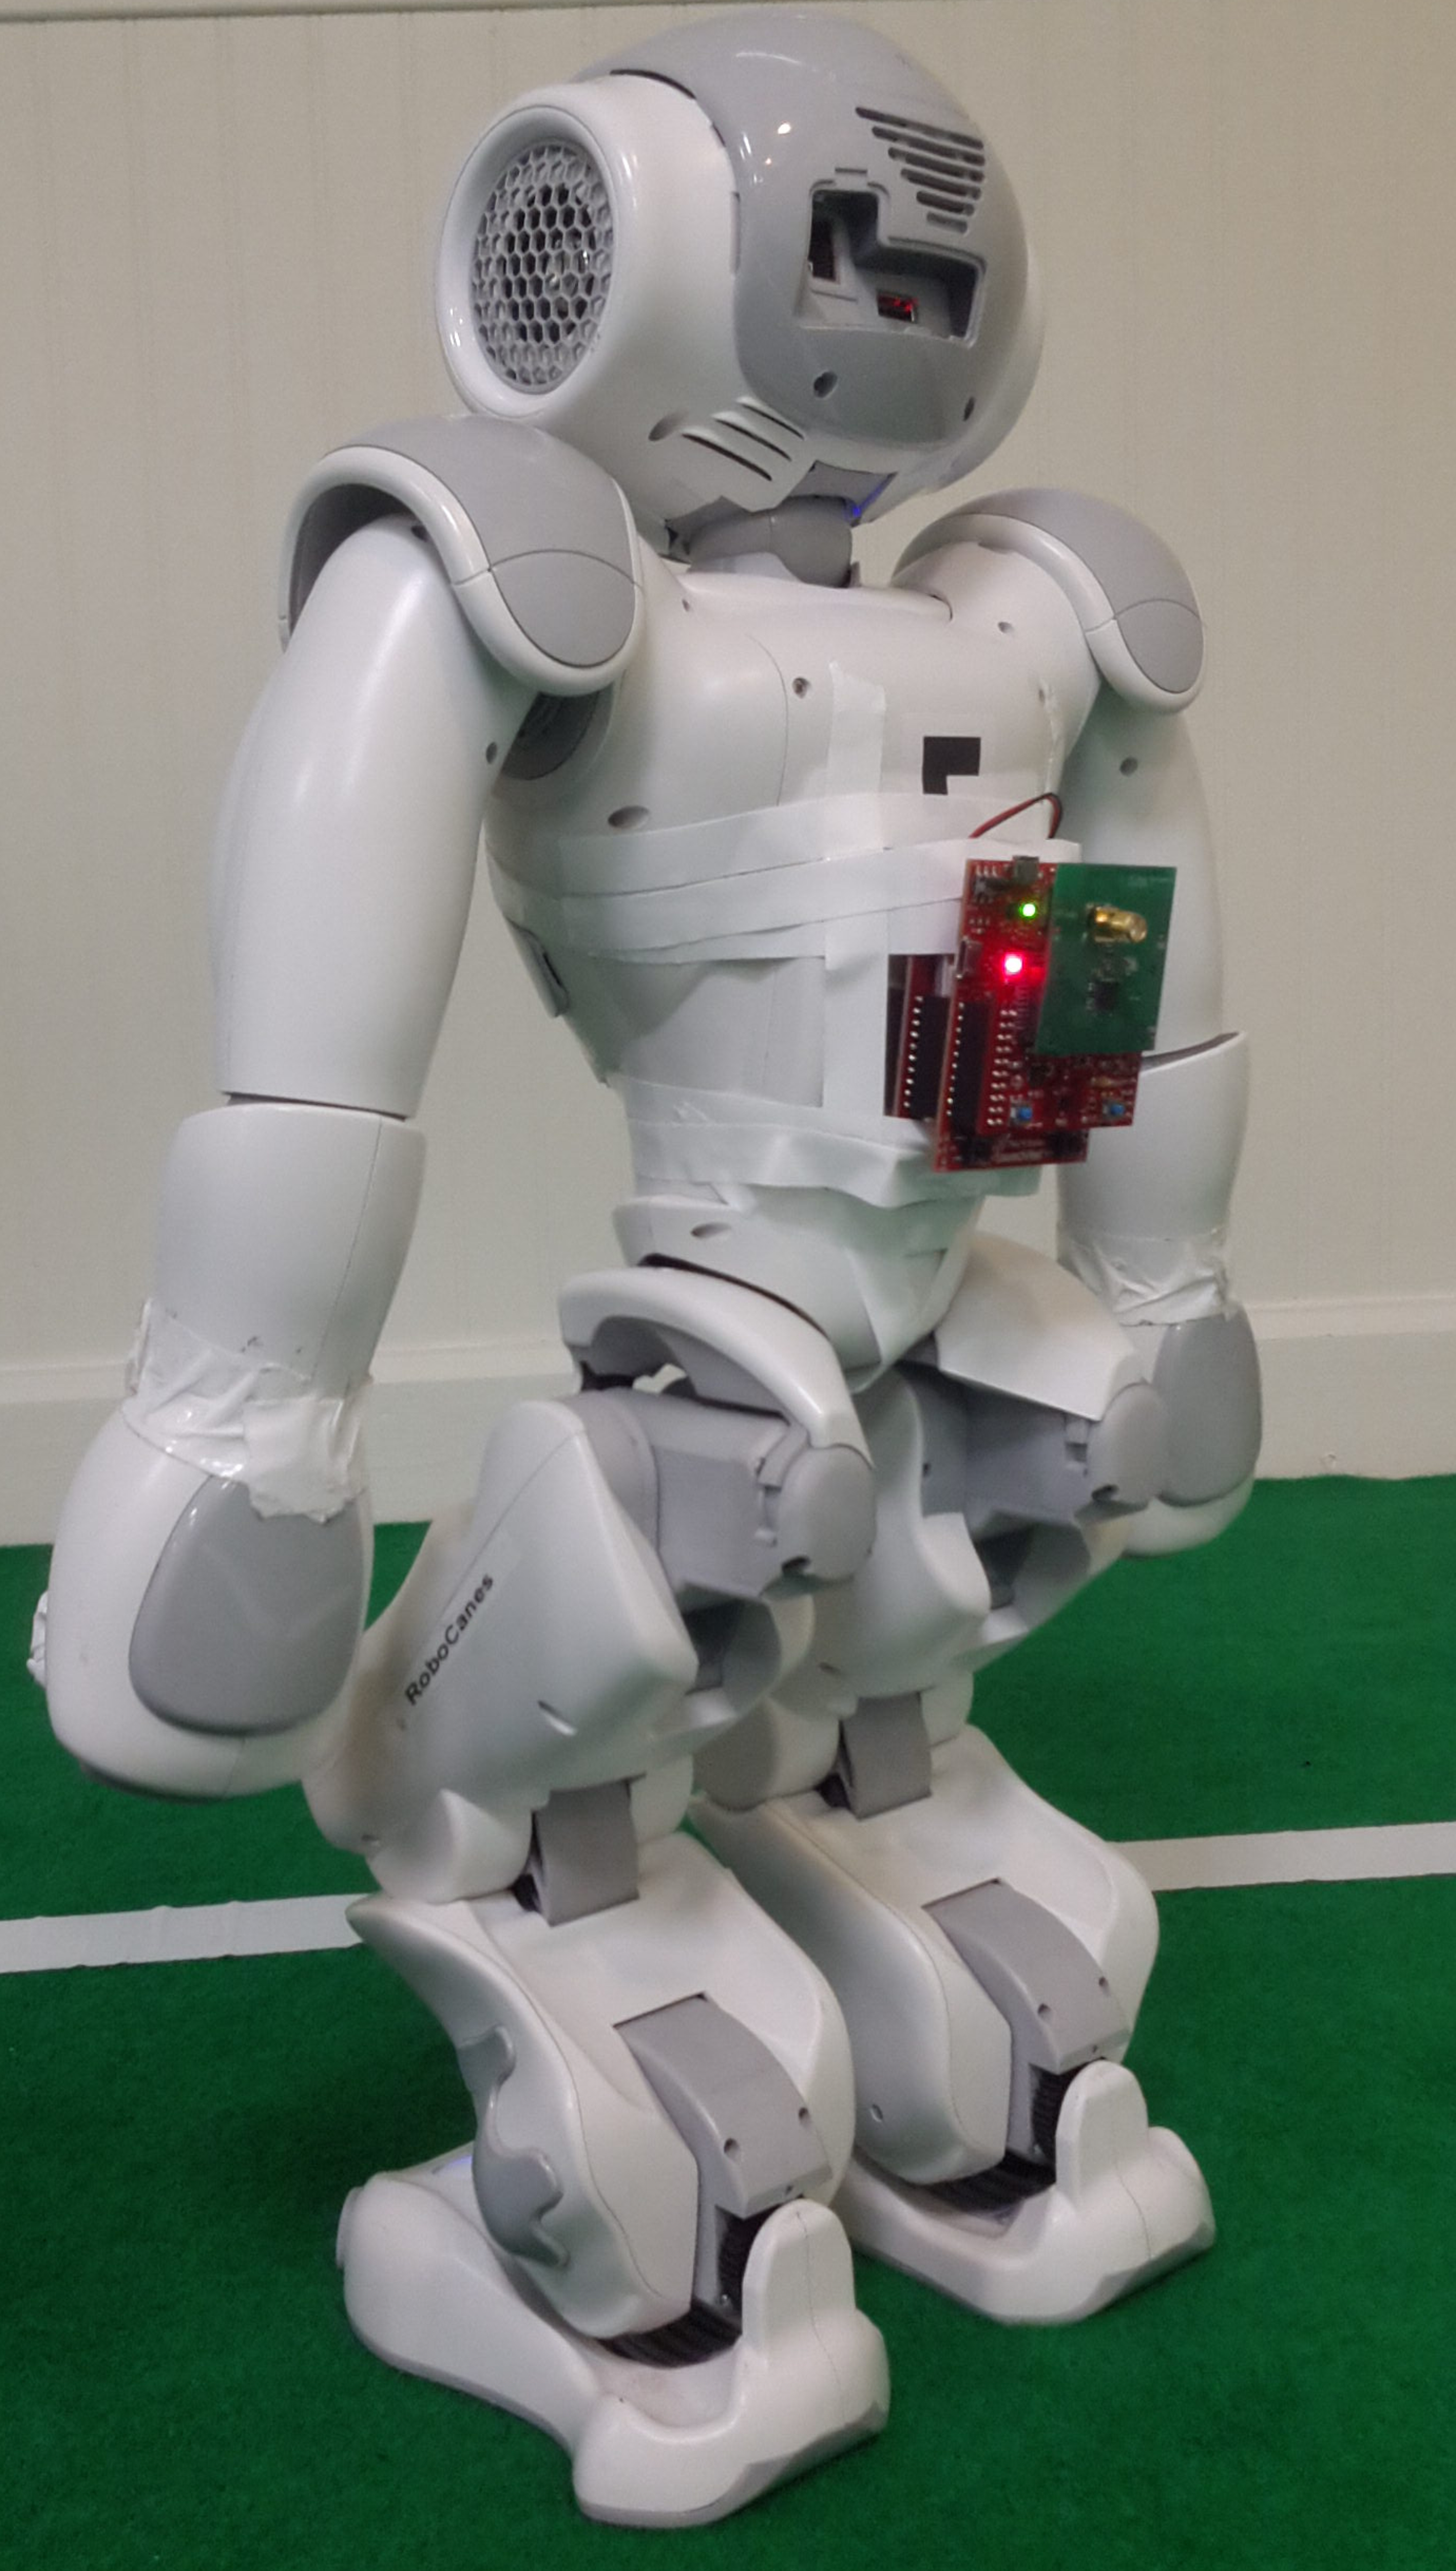
\includegraphics[width=0.62\linewidth]{figures/robot_figure}
			%\caption{7 Vs 7}\label{fig:timeIndiPlot}
		%\end{tcolorbox}
		\endminipage
	\end{figure}

	

}


%%%%%%%%%%%%%%%%%%%%%%%%%%%%%%%%%%%%%%%%%%%%%%%%%%%%%%%%%%%%%


\frame{
	\frametitle{Our Approach and Contributions}
	\setbeamercovered{transparent} 
	\begin{tcolorbox}[colback=green!5,colframe=darkgreen!90!black,title=Framework for Scheduling Processes]
		\begin{itemize}
				\item Collect process dependence descriptions.
				\item Create directed acyclic graph. 
				\item Create process execution schedule using topological sorting.
				\item ``$\mu$Energia'': \url{http://muenergia.saminda.org}
			\end{itemize}
	\end{tcolorbox}
	
}





%%%%%%%%%%%%%%%%%%%%%%%%%%%%%%%%%%%%%%%%%%%%%%%%%%%%%%%%%%%%%

\frame{
	\frametitle{Software Overview}
	\setbeamercovered{transparent} 
%\begin{tcolorbox}[colback=white!5,colframe=darkgreen!90!black]
\begin{figure}
    \centering
    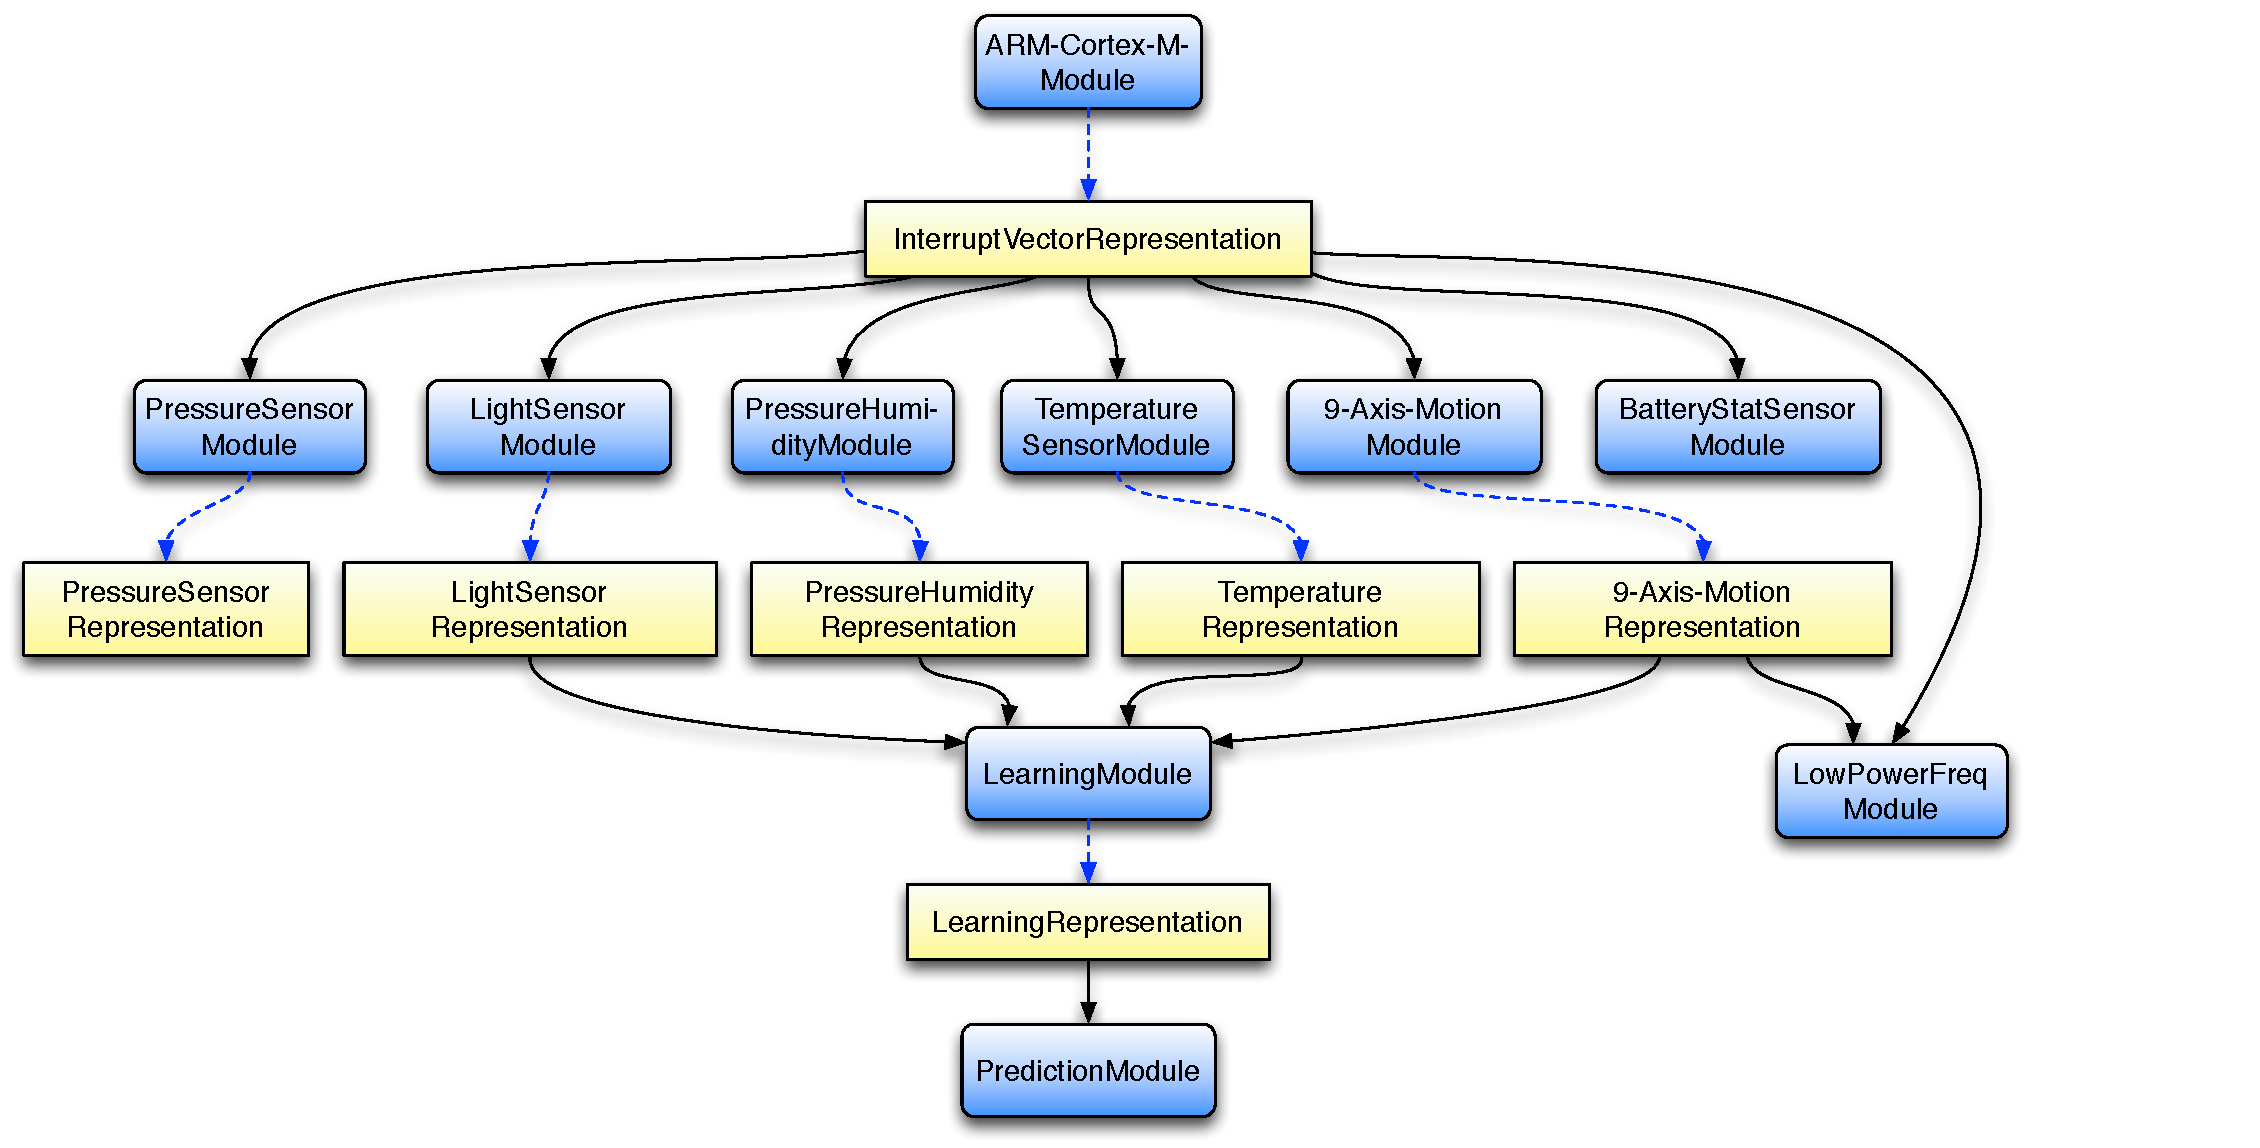
\includegraphics[width=\textwidth]{figures/graph_structure_def-crop3}
\end{figure}
%\end{tcolorbox}


}
%%%%%%%%%%%%%%%%%%%%%%%%%%%%%%%%%%%%%%%%%%%%%%%%%%%%%%%%%%%%%


\frame{
	\frametitle{Example Traces}
	\framesubtitle{Human (Left) and Robot (Right) Falling Forward}
	\setbeamercovered{transparent} 
	\begin{figure}[!ht]
		\minipage{0.48\textwidth}
		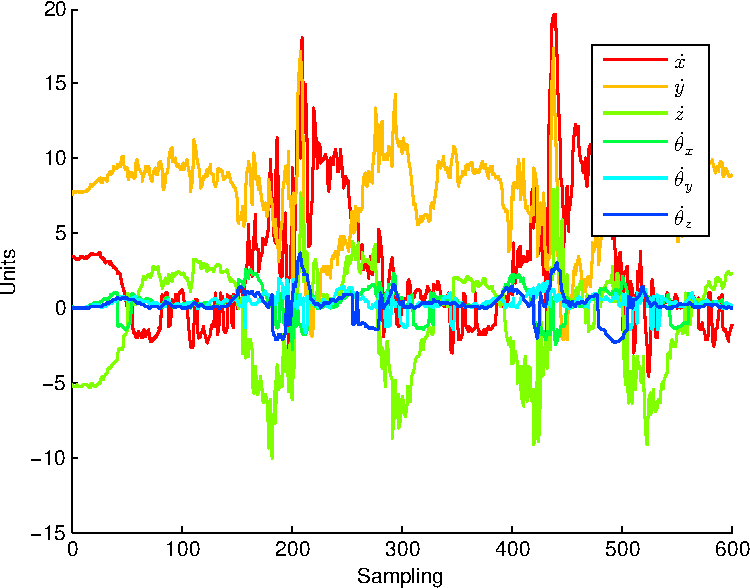
\includegraphics[width=\linewidth]{plots/human_falling-crop.pdf}
			% why 6 axis not 9 axis
			%\caption{5 Vs 5}\label{fig:timePlot}
		\endminipage \hfill
		\minipage{0.48\textwidth}
		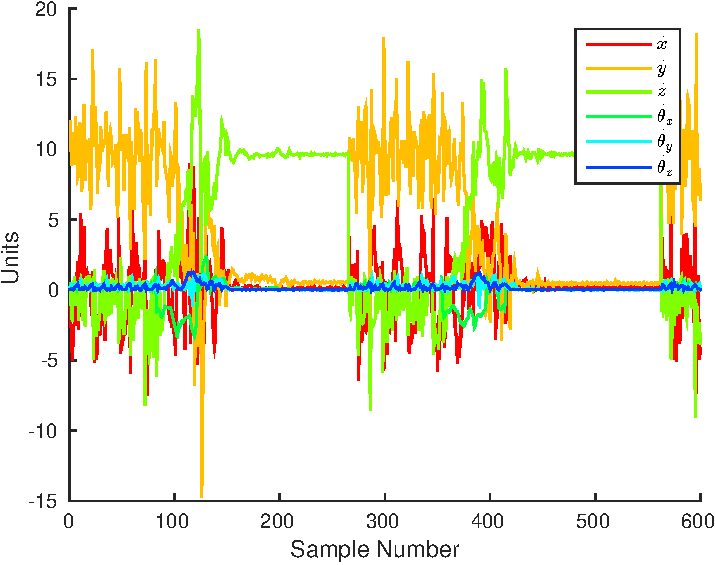
\includegraphics[width=\linewidth]{plots/robot_fallen_forward2-crop.pdf}
		\endminipage
	\end{figure}

\begin{tcolorbox}[colback=green!5,colframe=darkgreen!90!black]
{\small \begin{itemize}
\item $\dot{x}, \dot{y}, \mbox{  and } \dot{z}$: accelerometer readings in $m/s^2$.
\item $\dot{\theta_x}, \dot{\theta_y}, \mbox{  and } \dot{\theta_z}$: gyroscope readings in 
$rad/s$.
\end{itemize}	} 
	  \end{tcolorbox} 	

}


%%%%%%%%%%%%%%%%%%%%%%%%%%%%%%%%%%%%%%%%%%%%%%%%%%%%%%%%%%%%%



\section{Evaluation \& Results}
\subsection{Feature Extraction}
\subsection{Experiments with a Human}
\subsection{Experiments with a NAO Robot}

\frame{
	\frametitle{Featues}
	\setbeamercovered{transparent} 
	
	\begin{tcolorbox}[colback=green!5,colframe=darkgreen!90!black,title=Feature Extraction]
	\begin{itemize}
			\item 50$Hz$ sampling rate. 
			\item For activity identification: 
			\begin{enumerate} 
			\item Window size of $400ms$ (20 	samples); and 
			\item Allowed 10 samples ($200ms$) to overlap between 
					windows. 
				\end{enumerate} 
				\item The selection of the window size is based on the observation that a transition 
				from routine  activities to a fall event 
				takes between $180-250ms$. 
				\item Thus, a window size of $400ms$ will include both fall event and 
				non-fall event data for classification
			\end{itemize}
	\end{tcolorbox}
	
	
}

%%%%%%%%%%%%%%%%%%%%%%%%%%%%%%%%%%%%%%%%%%%%%%%%%%%%%%%%%%%%%
\frame{
	\frametitle{Evaluation \& Results}
	\setbeamercovered{transparent}
	\begin{tcolorbox}[colback=green!5,colframe=darkgreen!90!black,title=Experiments with a Human]
Twelve motions: 
			
			\begin{table}[!ht]
				
				\label{tab:human-logistic-class}
				\centering
				\scalebox{0.65}{
					\begin{tabular} {| l | c | c | c| c|| c| c| c| c|}
						\hline
						& \multicolumn{4}{c||}{\bf Logistic regression} & \multicolumn{4}{c|}{\bf 
						SVM classification} \\ 
						\hline
						{\bf Activity} & {\bf  TP}  &	{\bf TN}  &	{\bf FP} &	{\bf FN}& {\bf  
						TP}  &	{\bf TN}  &	{\bf FP} &	{\bf FN} \\ 
						\hline
						Walking forward	& 91\%	& 90\%	& 10\%	& 9\% & 96\%	& 93\%	& 7\%	& 
						4\% \\ \hline
						Walking backward	& 82\%	& 86\%	& 14\%	& 18\% & 81\%	& 84\%	& 16\%	
						& 19\% \\ \hline
						Walking left 	& 86\%	& 86\%	& 14\%	& 14\% & 89\%	& 90\%	& 10\%	& 
						11\% \\ \hline
						Walking right 	& 86\%	& 86\%	& 14\%	& 14\% & 89\%	& 90\%	& 10\%	& 
						11\% \\ \hline
						Falling forward	& 94\%	& 93\%	& 7\%	& 6\% & 96\%	& 93\%	& 7\%	& 
						4\%	 \\ \hline
						Falling Backward	& 84\%	& 88\%	& 12\%	& 16\%	& 84\%	& 87\%	& 13\%	
						& 16\% \\ \hline
						Falling left	& 92\%	& 91\%	& 9\%	& 8\%	& 93\%	& 93\%	& 7\%	& 
						7\% \\ \hline
						Falling Right	& 92\%	& 91\%	& 9\%	& 8\%	& 92\%	& 93\%	& 7\%	& 
						8\% \\ \hline
						Marching	& 91\%	& 90\%	& 10\%	& 9\%	& 95\%	& 93\%	& 7\%	& 5\% 
						\\ \hline
						Rotate counter-clockwise	& 91\%	& 89\%	& 11\%	& 9\%	& 93\%	& 91\%	
						& 9\%	& 7\%	 \\ \hline
						Rotate clockwise	& 92\%	& 89\%	& 11\%	& 8\%	& 94\%	& 91\%	& 9\%	
						& 6\% \\ \hline
						Stand to seat	& 96\%	& 92\%	& 8\%	& 4\%	& 96\%	& 92\%	& 8\%	& 
						4\%	 \\ \hline
					\end{tabular}
				}
				%\caption{Logistic regression and SVM classifications.}
			\end{table}
	
	\end{tcolorbox} 
	
	
}


%%%%%%%%%%%%%%%%%%%%%%%%%%%%%%%%%%%%%%%%%%%%%%%%%%%%%%%%%%%%%
\frame{
	\frametitle{Evaluation \& Results}
	\setbeamercovered{transparent} 
	
	\begin{figure}[!ht]
			\centering
%			\minipage{0.3\textwidth}
%						%\begin{tcolorbox}[colback=white!5,colframe=darkgreen!90!black]
%							\centering 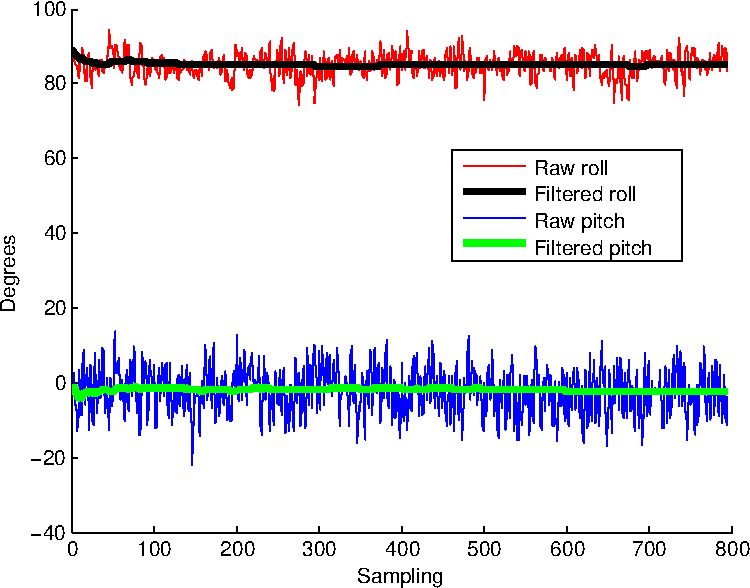
\includegraphics[width=\linewidth]{figures/plot1-crop}
%							%\caption{5 Vs 5}\label{fig:timePlot}
%						%\end{tcolorbox}
%			\endminipage 
			\minipage{0.32\textwidth}
			%\begin{tcolorbox}[colback=white!5,colframe=darkgreen!90!black]
				\centering 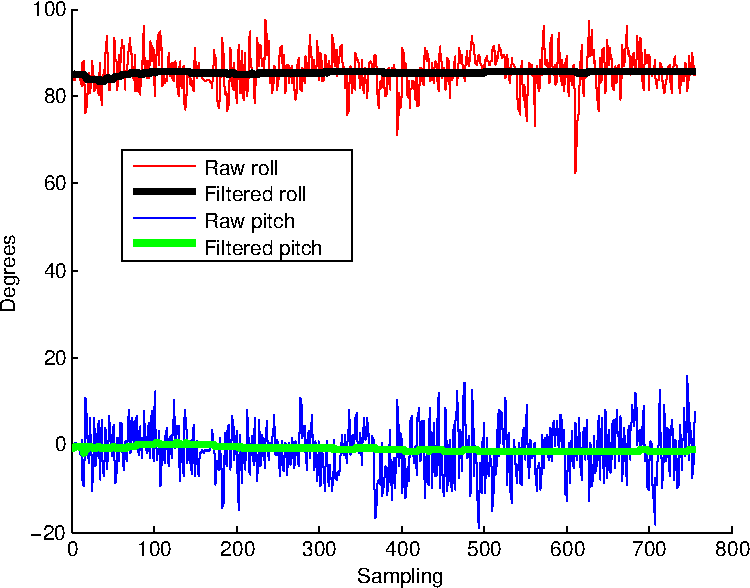
\includegraphics[width=\linewidth]{figures/plot5-crop}
				%\caption{7 Vs 7}\label{fig:timeIndiPlot}
			%\end{tcolorbox}
			\endminipage
			\minipage{0.32\textwidth}\hfill
			%\begin{tcolorbox}[colback=white!5,colframe=darkgreen!90!black]
				\centering 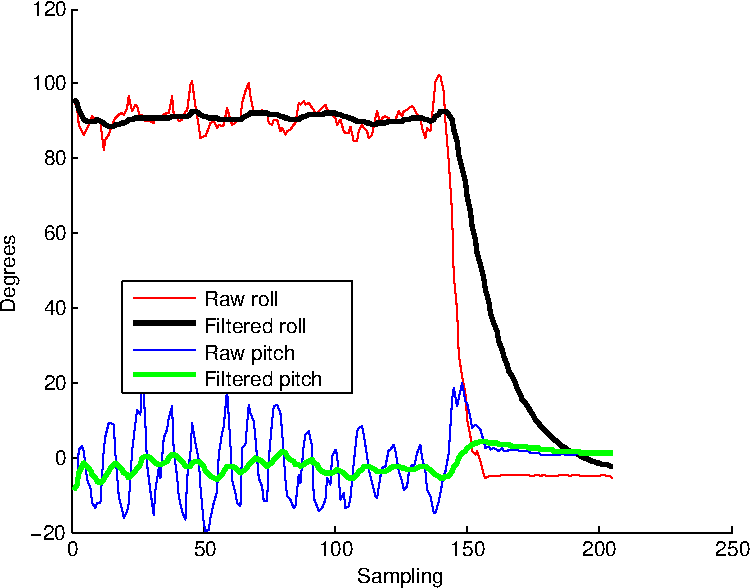
\includegraphics[width=\linewidth]{figures/plot1_fallen-crop}
				%\caption{5 Vs 5}\label{fig:timePlot}
			%\end{tcolorbox}
			\endminipage 
			\minipage{0.32\textwidth}
			%\begin{tcolorbox}[colback=white!5,colframe=darkgreen!90!black]
				\centering 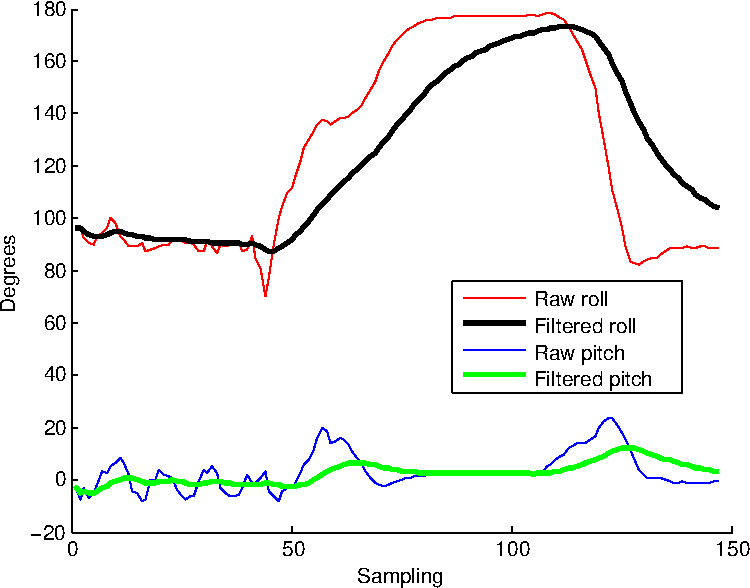
\includegraphics[width=\linewidth]{figures/plot2_fallen-crop}
				%\caption{7 Vs 7}\label{fig:timeIndiPlot}
			%\end{tcolorbox}
			\endminipage
		\end{figure}
			%kalman filter for euler angles.
	{\tiny \begin{tcolorbox}[colback=green!5,colframe=darkgreen!90!black,title=Kalman Filtering]
	\begin{itemize}
				\item Threshold-based decision making.
				\item Roll: $[90\pm15^{\circ}]$ \&\& Pitch: $[0\pm15]^{\circ}$ $\rightarrow$ normal state (100\%).
				\item Roll $< 60^{\circ}$ $\rightarrow$ falling forward. 
				\item Roll $< 100^{\circ}$ $\rightarrow$ falling backward.
				\item Pitch $< -50^{\circ}$ $\rightarrow$ falling left side.
				\item Pitch $> 50^{\circ}$ $\rightarrow$ falling right side. 
			\end{itemize}
	\end{tcolorbox}}
	
	
}

%%%%%%%%%%%%%%%%%%%%%%%%%%%%%%%%%%%%%%%%%%%%%%%%%%%%%%%%%%%%%
\subsubsection*{Experiments with a NAO Robot}
%\frame{
%	\frametitle{Evaluation Results}
%	\setbeamercovered{transparent} 
%	\begin{block}{Kalman Filtering}
%		\begin{figure*}
%			\includegraphics[width=0.25\textwidth]
%				{figures/plot1-crop}
%			\includegraphics[width=0.25\textwidth]
%				{figures/plot5-crop}
%			\includegraphics[width=0.25\textwidth]
%				{figures/plot1_fallen-crop}
%			\includegraphics[width=0.25\textwidth]
%				{figures/plot2_fallen-crop}
%			\caption{Figures (a--b) show the roll and pitch angles (raw and filtered) for normal 
%				behaviors marching in place and walking backward. Figures (c--d) show the raw and 
%filtered roll 
%				and pitch angles for fallen forward and backwards states of NAO humanoid robot.}
%			\label{fig:normalFallenBehavior}
%		\end{figure*}
%	\end{block}
%}

%%%%%%%%%%%%%%%%%%%%%%%%%%%%%%%%%%%%%%%%%%%%%%%%%%%%%%%%%%%%%
\frame{
	\frametitle{Evaluation \& Results}
	\setbeamercovered{transparent}
	
	\begin{tcolorbox}[colback=green!5,colframe=darkgreen!90!black,title=Experiments with a NAO 
	Robot]
Eleven motions: 
			\begin{table}[!ht]
				
				\label{tab:robot-logistic-class}
				\centering
				\scalebox{0.65}{
					\begin{tabular} {| l | c | c | c| c|| c| c| c| c|}
						\hline
						& \multicolumn{4}{c||}{\bf Logistic regression} & \multicolumn{4}{c|}{\bf 
						SVM classification} \\ 
						\hline
						{\bf Activity} & {\bf  TP}  &	{\bf TN}  &	{\bf FP} &	{\bf FN}& {\bf  
						TP}  &	{\bf TN}  &	{\bf FP} &	{\bf FN} \\ 
						\hline
						Walking forward	& 91\%	& 90\%	& 10\%	& 9\% & 93\%	& 91\%	& 9\%	& 7 
						\% \\ \hline
						Walking backward	& 90\%	& 90\%	& 10\%	& 10\% & 93\%	& 91\%	& 9\%	
						& 7\% \\ \hline
						Walking left 	& 92\%	& 90\%	& 10\%	& 8\%  & 94\%	& 90\%	& 10\%	& 
						6\% \\ \hline
						Walking right 	& 89\%	& 90\%	& 10\%	& 11\% & 90\%	& 91\%	& 9\%	& 
						10\% \\ \hline
						Falling forward	& 94\%	& 93\%	& 7\%	& 6\%	& 98\%	& 93\%	& 7\%	& 
						2\% \\ \hline
						Falling Backward	& 94\%	& 93\%	& 7\%	& 6\%	 & 98\%	& 93\%	& 7\%	
						& 2\% \\ \hline
						Falling left	& 95\%	& 93\%	& 7\%	& 5\%	& 99\%	& 94\%	& 6\%	& 
						1\% \\ \hline
						Falling Right	& 94\%	& 93\%	& 7\%	& 6\%	& 98\%	& 93\%	& 7\%	& 
						2\%	 \\ \hline
						Marching	& 91\%	& 89\%	& 11\%	& 9\%	& 90\%	& 91\%	& 11\%	& 
						10\%	 \\ \hline
						Rotate counter-clockwise	& 97\%	& 92\%	& 8\%	& 3\%	& 97\%	& 93\%	
						& 7\%	& 3\%	 \\ \hline
						Rotate clockwise	& 98\%	& 92\%	& 8\%	& 2\%	& 96\%	& 93\%	& 7\%	
						& 4\%	 \\ \hline
					\end{tabular}
				}
				%\caption{Logistic regression  and SVM classifications.}
			\end{table}
	\end{tcolorbox}
	
}

%%%%%%%%%%%%%%%%%%%%%%%%%%%%%%%%%%%%%%%%%%%%%%%%%%%%%%%%%%%%%

\section{Conclusion \& Future Work}

\frame{
	\frametitle{Conclusion \& Future Work}
	\setbeamercovered{transparent} 
	\begin{tcolorbox}[colback=green!5,colframe=darkgreen!90!black,title=Conclusion \& Future Work]
	\begin{itemize}
			 \item	Learn and predict different activities for humans and robots.
			\item Framework  for	embedded devices.
			\item Detect normal activities and fall events with high accuracy.
			\item Sensor network.
			\item To use the devices in other domains. 
			\end{itemize}
	\end{tcolorbox}
	
}


%%%%%%%%%%%%%%%%%%%%%%%%%%%%%%%%%%%%%%%%%%%%%%%%%%%%%%%%%%%%%

%\section{*Conclusion \& Future Work}
%\subsubsection*{*Conclusion \& Future Work}

\frame{
	\frametitle{}
	\setbeamercovered{transparent}
	\begin{tcolorbox}[colback=green!5,colframe=darkgreen!90!black]
	  \center \huge Thank You
	  \end{tcolorbox} 
}

%%%%%%%%%%%%%%%%%%%%%%%%%%%%%%%%%%%%%%%%%%%%%%%%%%%%%%%%%%%%%

%\section{*Conclusion \& Future Work}
%\subsubsection*{*Conclusion \& Future Work}

\section{Conclusion \& Future Work}

\frame{
	\frametitle{~}
	\setbeamercovered{transparent} 
	\begin{tcolorbox}[colback=green!5,colframe=darkgreen!90!black,title=Related Work]
	\begin{itemize}
			 \item	Detection of fall incidences among the elderly people \cite{ojetola2011fall}.
			 \item  Classification of behaviors and postures \cite{baek2013real}.
			 \item  Detection of events that cause trauma and disabilities \cite{leone2013supervised}.
			 \item  Activity detection systems 
			\cite{Bao04activityrecognition,dumitrache2013fall,kumarwearable,krishnan2014activity,gao2014evaluation,alvarez2015evaluating}.
			\item Detection of fall and damage reduction mechanism for humanoid robots 
			\cite{moya2014fall}.
			\item Activity detection with smart-phones
			\cite{bai2013recognition,steidl2012fall,DernbachDKTC12,Shen2015390}.
			\end{itemize}
	\end{tcolorbox}	
}


\begin{frame}[allowframebreaks]
	\tiny
	\bibliography{references}
	\bibliographystyle{alpha}
	\normalsize
\end{frame}


\end{document}